\section{Wykonanie}
\label{sec:wykonanie}

\subsection{Prototyp na blokach Simulink}

Stworzyliśmy w pełni działający układ korzystając z niezależnych
bloków z pakietów dostarczanych przez Simulink. Miało to ułatwić wprowadzanie
zmian parametrów sterujących podzespołami i dodatkowych punktów kontrolnych
wewnątrz układu. Schemat prototypu znajduje się na rysunku
\ref{fig:pll_prototyp} na~stronie~\pageref{fig:pll_prototyp}.

\begin{figure}[h]
    \centering
    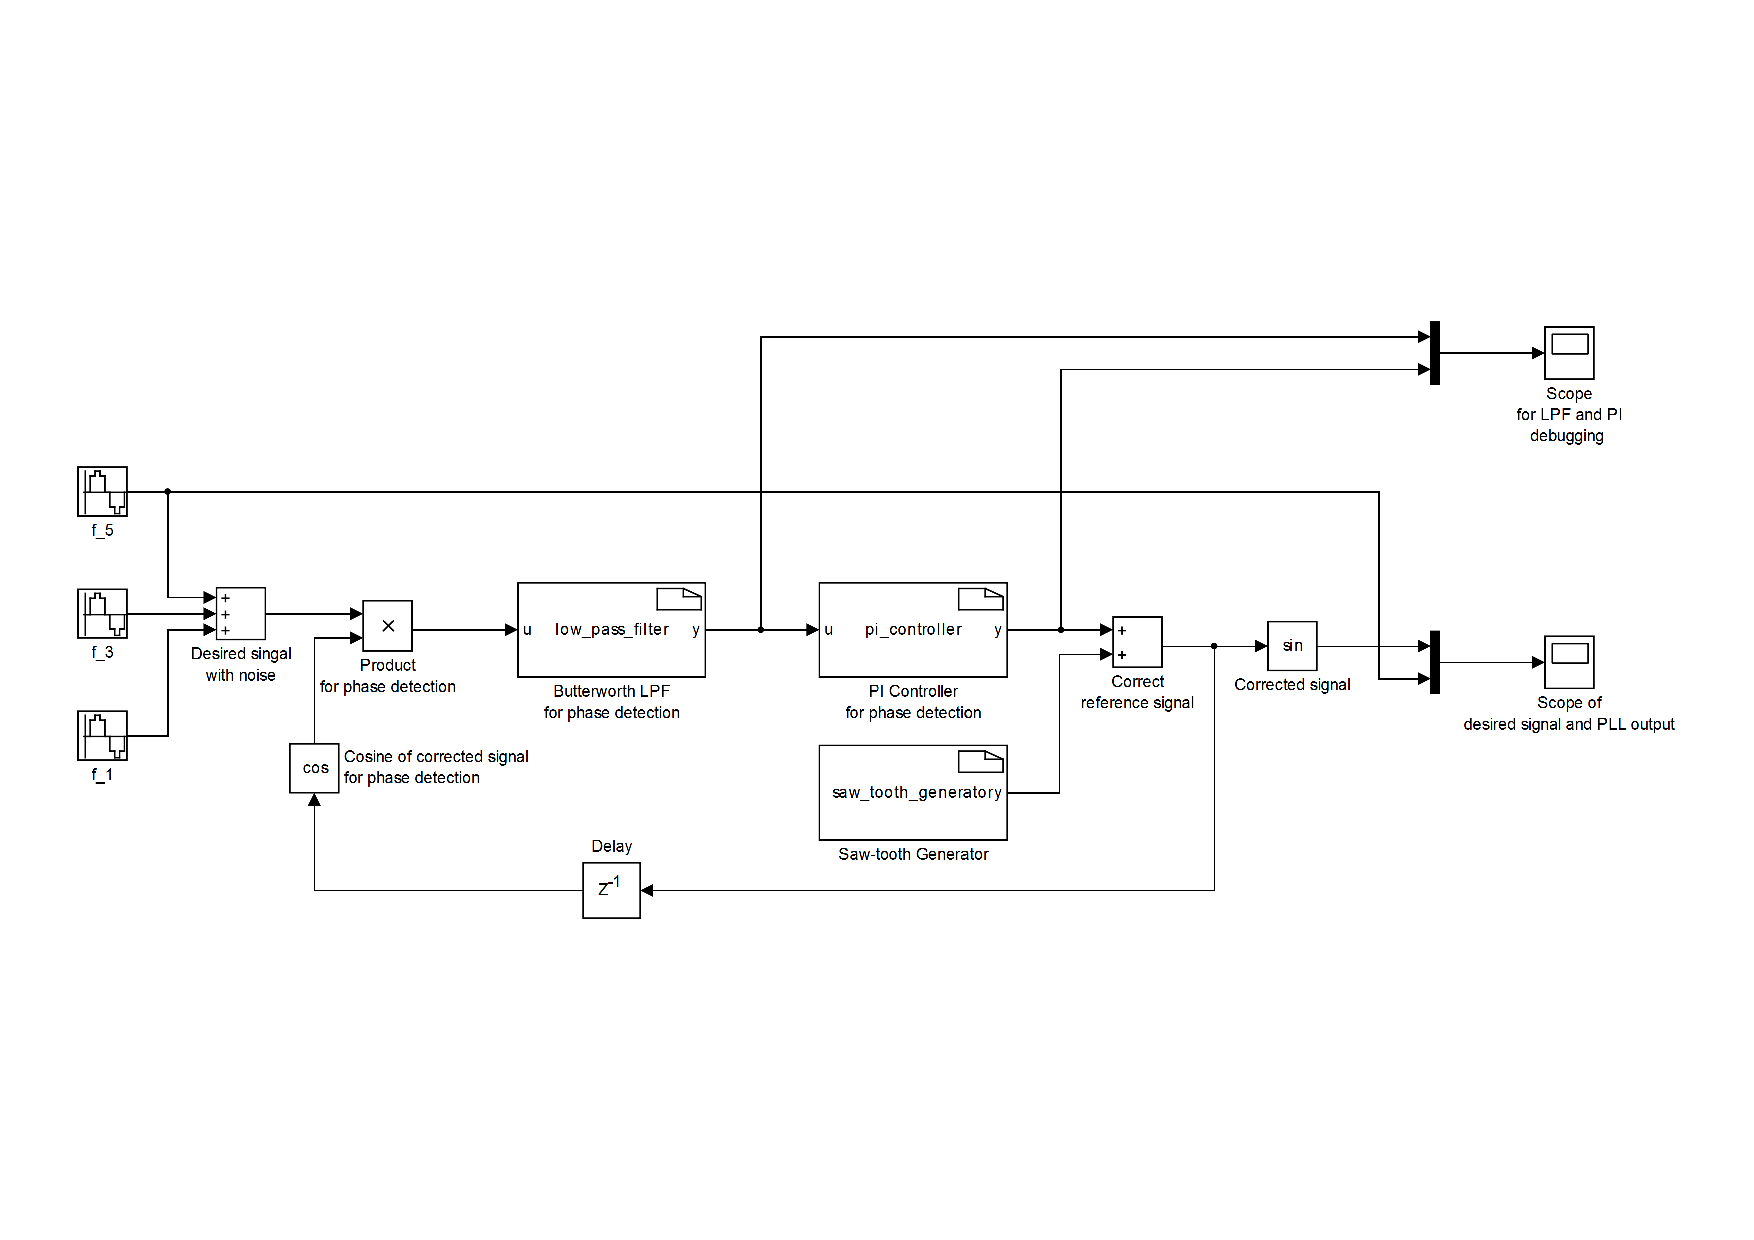
\includegraphics[angle=180, trim=5cm 1cm 5cm 1cm, scale=0.8]{./figury/schemat-prototypu}
    \caption{Schemat prototypu układu PLL zbudowany z niezależnych bloków z
        pakietów Simulink.}
    \label{fig:pll_prototyp}
\end{figure}

Układ jest zbudowany identycznie z modelem zaprezentowanym w czasie zajęć
laboratoryjnych. Szczegóły implementacyjne podzespołów i dobrane parametry są
identyczne ze szczegółami modelu końcowego opisanego
w~sekcji~\ref{sec:pll}.


\subsection{Wersja końcowa zaimplementowana w C}
\label{sec:pll}
Układ w wersji końcowej składa się z jednego bloku łączącego podzespoły z
prototypu wewnątrz swojej implementacji w C. Schemat układu PLL w wersji
końcowej znajduje się na stronie \pageref{fig:pll}.

\noindent Kod C bloku \texttt{PLL} realizujący cały układ jest przedstawiony
poniżej na listingu \ref{lst:pll_kod}. W następnych sekcjach opisane są
szczegółowo funkcje realizujące kolejne podzespoły układu.

\begin{lstlisting}[caption={Implementacja układu PLL w C.}, label=lst:pll_kod]
// blok PLL
static double feedback_in = 1.0;

lpf_out[0] = low_pass_filter(signal_in[0] * feedback_in);
pi_ctrl_out[0] = pi_controller(lpf_out[0]);
saw_out[0] = saw_tooth_generator();

pll_out[0] = sin(saw_out[0] + pi_ctrl_out[0]);
feedback_in = cos(saw_out[0] + pi_ctrl_out[0]);
\end{lstlisting}

\begin{figure}[h]
    \centering
    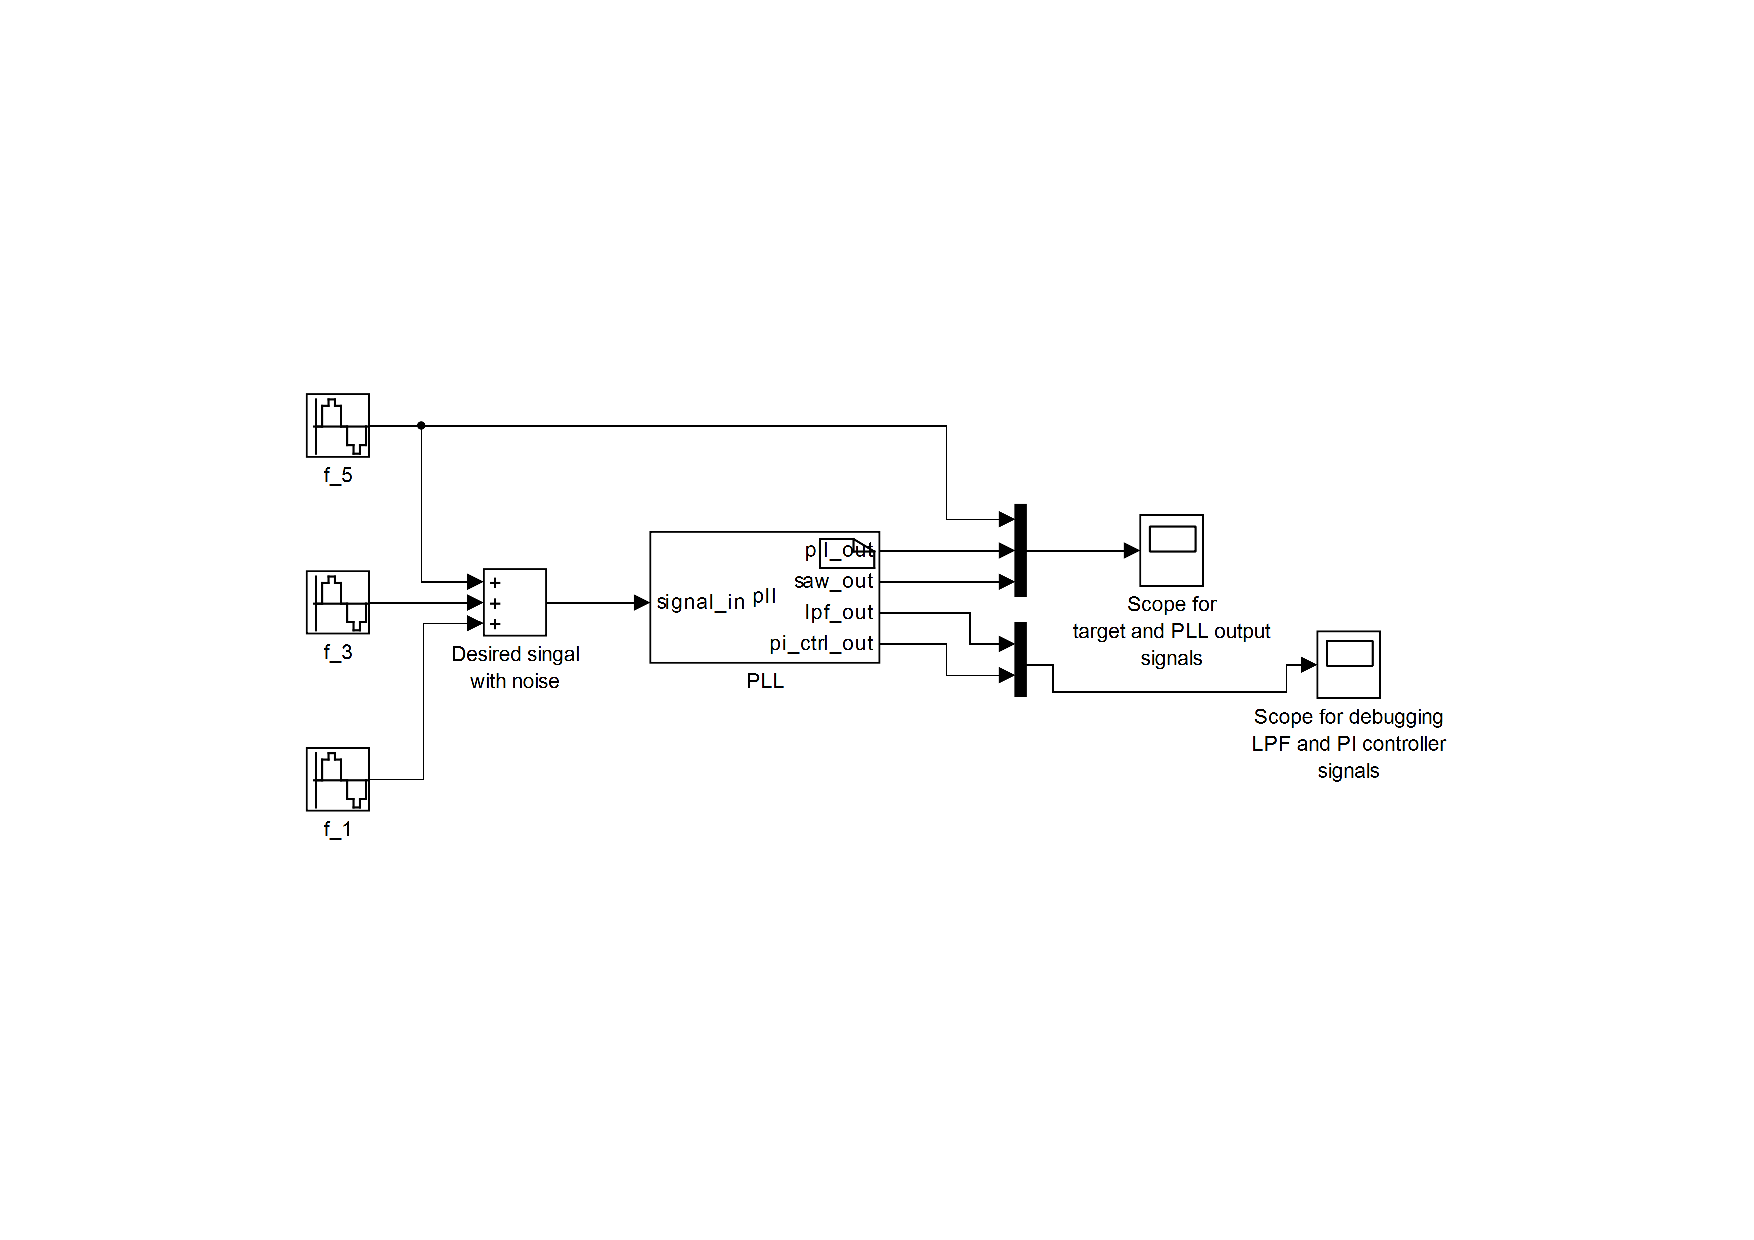
\includegraphics[angle=180, trim=5cm 5cm 5cm 5cm]{./figury/schemat-koncowy}
    \caption{Schemat układu PLL zaimplementowanego w C.}
    \label{fig:pll}
\end{figure}

\subsubsection{Detektor przesunięcia fazy}
Został zaimplementowany zgodnie z wytycznymi z zajęć. Zasada działania jest
prosta. Iloczyn wartości sygnałów referencyjnego i porównywanego jest podawany
na wejście filtra dolnoprzepustowego. Pozwala to z wystarczająco dobrym
przybliżeniem wyznaczyć wartość przesunięcia fazowego.

Filtr dolnoprzepustowy wykorzystany w układzie został wygenerowany za pomocą
programu WinFilter w wersji 0.8 \cite{filtr_site}. Do naszych potrzeb
najlepszy okazał się filtr dolnoprzepustowy Butterwortha czwartego rzędu.
Parametry operacyjne filtru dobraliśmy eksperymentalnie. Ich wartości są
wypisane w tabeli \ref{tab:filtr_parametry}.

\begin{table}[h]
    \centering
    \begin{tabular}{lr}
        \toprule
        \textbf{Parametr} & \textbf{Wartość} \\
        \midrule
        Model filtru & Butterworth \\
        Rząd filtru & 4 \\
        Częstotliwość próbkowania (narzucona) & 10 kHz \\
        Częstotliwość odcięcia & 0,025 kHz \\
        \bottomrule
    \end{tabular}
    \caption{Parametry operacyjne filtru dolnoprzepustowego wchodzącego w skład detektora fazy.}
    \label{tab:filtr_parametry}
\end{table}

\noindent Funkcjonalność filtru jest zrealizowana w jednej funkcji
\texttt{low\_pass\_filter}. Jej definicja znajduje się w listingu
\ref{lst:filtr_kod}. Jako jedyny parametr przyjmuje wartość nowej próbki
sygnału. Zwraca wartość sygnału po przefiltrowaniu.

\begin{lstlisting}[
    caption={Implementacja filtru dolnoprzepustowego wchodzącego w skład dektora fazy.},
    label=lst:filtr_kod
]
// low_pass_filter.c
#define NCoef 4

double low_pass_filter(double newSample) {
    double ACoef[NCoef+1] = {
        0.00000000378517015213,
        0.00000001514068060852,
        0.00000002271102091279,
        0.00000001514068060852,
        0.00000000378517015213
    };

    double BCoef[NCoef+1] = {
        1.00000000000000000000,
        -3.95895331864708360000,
        5.87770027353614570000,
        -3.87853054905173390000,
        0.95978365381149922000
    };

    static double y[NCoef+1]; // output samples
    static double x[NCoef+1]; // input samples
    int n;

    // shift the old samples
    for (n = NCoef; n > 0; n--) {
       x[n] = x[n-1];
       y[n] = y[n-1];
    }

    // calculate the new output
    x[0] = newSample;
    y[0] = ACoef[0] * x[0];
    for (n = 1; n <= NCoef; n++)
        y[0] += ACoef[n] * x[n] - BCoef[n] * y[n];

    return y[0];
}
\end{lstlisting}

\subsubsection{Kontroler proporcjonalny-integrujący}
\label{sec:pi}
Wyjście z detektora fazy jest podawane na wejście kontrolera propocjonalnego-
integrującego. Jest on realizowany przez funkcję \texttt{pi\_controller}, która
przyjmuje wartość kolejnej próbki sygnału i zwraca sygnał po przeprowadzeniu obu
operacji. Parametry kontrolera również zostały dobrane eksperymentalnie, zgodnie
ze wskazówkami z konsultacji. Wybrane wartości parametrów są zestawione w
tabeli \ref{tab:pi_parametry}. Tak dobrane parametry pozwalają na najszybsze
zsynchronizowanie układu dla przypadku opisanego w naszym zadaniu
(vide sekcja~\ref{sec:zadanie}).

\begin{table}[h]
    \centering
    \begin{tabular}{lc}
        \toprule
        \textbf{Parametr} & \textbf{Wartość} \\
        \midrule
        Waga członu integrującego & 0,0075 \\
        Waga członu proporcjonalnego & 0,3000 \\
        \bottomrule
    \end{tabular}
    \caption{Parametry operacyjne kontrolera PI przetwarzającego sygnał detektora fazy.}
    \label{tab:pi_parametry}
\end{table}

\noindent Implementacja funkcji realizującej kontroler PI jest identyczna z
implementacją wykonaną podczas pierwszych zajęć laboratoryjnych. Jest
przedstawiona poniżej na listingu \ref{lst:pi_kod}.

\begin{lstlisting}[
    caption={Implementacja kontrolera PI przetwarzającego sygnał z detektora fazy.},
    label=lst:pi_kod
]
// pi_controller.c
#define K_i 0.0075
#define K_p 0.3

double pi_controller(double u)
{
    static double u_p, y_p;

    double y = (K_p + K_i) * u - K_p * u_p + y_p;
    y_p = y;
    u_p = u;
    return y;
}
\end{lstlisting}

\subsubsection{Generator sygnału referencyjnego piło\dywiz kształtnego}
\label{sec:generator}
Sygnał z detektora przesunięcia fazy, przetworzony przez kontroler PI jest
dodawany jako korekcja do sygnału referencyjnego nadawanego przez generator
sygnału piło\dywiz kształtnego. Zgodnie z wytycznymi zadania generator na
wyjściu podawał sygnał o częstotliwości $f_{ref} = \unit[250]{Hz}$ i amplitudzie
$|s_{ref}| = 2\pi$.

\noindent Jest on realizowany przez funkcję \texttt{saw\_tooth\_generator}, która
nie przyjmuje argumentów i zwraca wartość kolejnych próbek sygnału
referencyjnego. Jej implementacja znajduje się
w~listingu~\ref{lst:generator_kod}.

\begin{lstlisting}[
    caption={Implementacja generatora sygnału referencyjnego.},
    label=lst:generator_kod
]
#define pi 3.1415926535897932384626433
#define f_smp 10000
#define f_target 250

double saw_tooth_generator()
{
    const double dy = 2*pi / f_smp * f_target;
    static double y = -2*pi / f_smp * f_target; // == -dy

    y = fmod(y+dy, 2*pi);

    return y;
}

\end{lstlisting}

\noindent Tak skorygowany sygnał jest podawany na wyjście układu oraz w
sprzężeniu zwrotnym na wejście detektora fazy.
